   
\documentclass[12pt]{amsart}
   \usepackage{geometry} % see geometry.pdf on how to lay out the page. There's lots.
   \geometry{a4paper} % or letter or a5paper or ... etc
   \usepackage{amsthm}
   \usepackage{float}
   \usepackage{graphicx}
   \newtheorem{prop}{Proposition}
   % \geometry{landscape} % rotated page geometry
   
   % See the ``Article customise'' template for come common customisations
   
   \title{Analytic Forms for Discrete-Time Clearance Price Optimization}
   \author{Ashwin Rao}
   \date{} % delete this line to display the current date
   
   %%% BEGIN DOCUMENT
   \begin{document}
   
   \maketitle 
   \section{Introduction}
   This is a brief article to derive analytic forms for Clearance Price Optimization when the Price actions can be performed at discrete and regular time steps. Clearance Price Optimization has some neat analytic forms for the case of continuous-time, eg: the landmark paper by Gallego and Ryzin in 1994. But discrete time-steps pose some challenges that we investigate in this article.    
   \section{Bellman Equation}
    The {\em State} at time $t \in \{0, 1, \ldots, T\}$ is the Inventory $I_t \in \mathbb{Z}_{\geq 0}$. The {\em Action} at time $t$ is the Price $p_t \in \mathbb{R}_{\geq 0}$ set at time $t$. Assume the probability mass function (PMF) of demand $k_t \in \mathbb{Z}_{\geq 0}$ at time $t$ has mean $f(p_t)$ and variance $g(p_t)$ for some given functions $f, g : \mathbb{R}_{\geq 0} \rightarrow \mathbb{R}_{\geq 0}$. The {\em Reward} at time $t$ is $p_t \cdot \min(k_t, I_t)$. Then, for all $t = 0, 1, \ldots, T-1$, we have the following Bellman Equation:
    
    $$V_t^*(I_t) = \max_{p_t} \{ \sum_{k_t=0}^{\infty} Pr[k_t; f(p_t), g(p_t)] \cdot (p_t \cdot \min(k_t, I_t) + V_{t+1}^*(\max(I_t - k_t, 0))) \}$$
    $$V_t^*(0) = 0, V_T^*(I_T) = 0$$
   
   As an example, consider the Poisson distribution for the PMF of demand given by Poisson mean $f(p_t) = \alpha \cdot e^{-\beta \cdot p_t}$ for all $t = 0, 1, \ldots, T-1$. Then,
   
    $$V_t^*(I_t) = \max_{p_t} \{ \sum_{k_t=0}^{I_t - 1} \frac {e^{-\alpha \cdot e^{-\beta \cdot p_t}} \cdot \alpha^{k_t} \cdot e^{-\beta \cdot k_t \cdot p_t}} {k_t!} \cdot (p_t \cdot k_t + V_{t+1}^*(I_t - k_t)) +  \sum_{k_t=I_t}^{\infty} \frac {e^{-\alpha \cdot e^{-\beta \cdot p_t}} \cdot \alpha^{k_t} e^{-\beta \cdot k_t \cdot p_t}} {k_t!} \cdot p_t \cdot I_t \}$$
    $$V_t^*(0) = 0, V_T^*(I_T) = 0$$
   
   For $t=T-1$, we take the derivative of the right hand side with respect to $p_{T-1}$ and set to 0. This enables us to solve for $p_{T-1}^*$ and $V_{T-1}^*$. Then we do the same for $t=T-2$ and proceed back in time to obtain $p_t^*$ and $V_t^*$ for all $t = 0, 1, \ldots T-1$.
   
   The above technique is easy for the case of deterministic demand.
   
   \section{Deterministic Case}
   Here we consider the case where demand is a deterministic function of price, denoted as $f : \mathbb{R}_{\geq 0} \rightarrow \mathbb{R}_{\geq 0}$ for each time step $t = 0, 1, \ldots T-1$. For the deterministic case, since demand at each time step $t$ is a continuous variable ($\in \mathbb{R}_{\geq 0}$), the inventory $I_t$ at time $t$ is a continuous variable ($\in \mathbb{R}_{\geq 0}$). Then, for all $t = 0, 1, \ldots T - 1$, we have the Bellman Equation:
   
   $$V_t^*(I_t) = \max_{p_t} \{ p_t \cdot \min(f(p_t), I_t) + V_{t+1}^*(\max(I_t - f(p_t), 0)) \}$$
   $$V_t^*(0) = 0,  V_T^*(I_T) = 0$$
  
  \subsection{Simplifying the Bellman Equation}
  We will assume that $f$ has an inverse $f^{-1} : \mathbb{R}_{\geq 0} \rightarrow \mathbb{R}_{\geq 0}$ and that $f$ is a monotonically decreasing function. Then, we have the following Proposition.
  \begin{prop}
  Optimal Pricing will not permit the demand at time $t$ to exceed the Inventory $I_t$ at time $t$, for all $t = 0, 1, \ldots, T-1$, i.e., $f(p_t^*) \leq I_t$ or equivalently, $p_t^* \geq f^{-1}(I_t)$.
  \end{prop}
  \begin{proof}
  Assume the contrary, that $f(p_t^*) > I_t$, or equivalently, $p_t^* < f^{-1}(I_t)$. Since demand $f(p_t^*)$ exceeds $I_t$, $I_{t+1} = 0$ and so, $V_{t+1}^*(I_{t+1}) = 0$. Therefore, $V_t^*(I_t) = p_t^* \cdot I_t < f^{-1}(I_t) \cdot I_t$. This says that a price of $f^{-1}(I_t)$ producing a demand of $I_t$ attains a {\em Reward} of  $f^{-1}(I_t) \cdot I_t$ at time step $t$ that exceeds the assumed optimal value function $V_t^*(I_t) \Rightarrow $ Reductio Ad Absurdum.
  \end{proof}
  
  An important consequence of this Proposition is that we can simplify the Bellman Equation:
  
  $$V_t^*(I_t) = \max_{p_t \geq f^{-1}(I_t)} \{ p_t \cdot f(p_t) + V_{t+1}^*(I_t - f(p_t)) \}$$
   $$V_t^*(0) = 0,  V_T^*(I_T) = 0$$

   \subsection{Exponential Price Function}
   Assume $f(p_t) = \alpha \cdot e^{-\beta \cdot p_t}$ for some given $\alpha, \beta \in \mathbb{R}_{> 0}$. Then,
   
   $$V_t^*(I_t) = \max_{p_t \geq \frac 1 \beta \log \frac \alpha {I_t}} \{ p_t \cdot \alpha \cdot e^{-\beta \cdot p_t}  + V_{t+1}^*(I_t - \alpha \cdot e^{-\beta \cdot p_t}) \}$$
   $$V_t^*(0) = 0, V_T^*(I_T) = 0$$
   
   We note that as $I_t \to 0$, $p_t^* \geq \frac 1 \beta \log \frac \alpha {I_t} \to \infty$, Demand under Optimal Price ($= \alpha \cdot e^{-\beta \cdot p_t^*}$) $\to 0$, and {\em Reward} under Optimal Price ($= p_t^* \cdot \alpha \cdot e^{-\beta \cdot p_t^*}$) $\to 0$.
   
   \subsection{Backward Recursion: Optimal Price/Value Function for $t = T-1$} 
   We start with time $t = T-1$ and solve the Bellman Equation by recursing back in time. The Bellman equation for time step $t = T-1$ is:
      
   $$V_{T-1}^*(I_{T-1}) = \max_{p_{T-1} \geq \frac 1 \beta \log \frac \alpha {I_{T-1}}} \{ \alpha \cdot p_{T-1} \cdot  e^{-\beta \cdot p_{T-1}} \}$$
   
   In order to perform the constrained maximization above, let us examine the function $h(x) = \alpha \cdot x \cdot e^{-\beta x}$ for all $x \in \mathbb{R}_{\geq 0}$.
   \begin{itemize}
   \item $h(0) = 0$
   \item $\lim_{x \to \infty} h(x) = 0$
   \item $h'(x) = \alpha \cdot e^{-\beta x} \cdot (1 - \beta x)$ and so, $h'(x) > 0$ for $x < \frac 1 \beta, h'(x) = 0$ for $x = \frac 1 \beta$, $h'(x) < 0$ for $x > \frac 1 \beta$
   % \item $h''(x) = \alpha \cdot \beta \cdot e^{-\beta x} \cdot (\beta x - 2)$ and so, $h''(x) < 0$ for $x < \frac 2 \beta, h''(x) = 0$ for $x = \frac 2 \beta$, $h''(x) < 0$ for $x > \frac 2 \beta$
   \end{itemize}

From the above analysis, we note that $h(x)$ has a single peak at $x = \frac 1 \beta$. If this peak occurs within the above-specified range for the price ($p_{T-1} \geq \frac 1 \beta \log \frac \alpha {I_{T-1}}$), then the optimal price is where the peak occurs ($= \frac 1 \beta$). Otherwise, the optimal price is the lower bound of this price range ($= \frac 1 \beta \log \frac \alpha {I_{T-1}}$). We also note that the above condition ($\frac 1 \beta \geq \frac 1 \beta \log \frac \alpha {I_{T-1}}$) can be succinctly expressed as: $I_t \geq \frac \alpha e$. Below, we summarize the Optimal Price and consequent Optimal Value Function for time step $t = T-1$:

$$
p_{T-1}^*(I_{T-1}) = 
\begin{cases}
\frac 1 \beta & \text{if } I_{T-1} \geq \frac \alpha e \\
\frac 1 \beta \log{ \frac \alpha {I_{T-1}}} & \text{if } I_{T-1} < \frac \alpha e\\
\end{cases}
$$

$$
V_{T-1}^*(I_{T-1}) = 
\begin{cases}
\frac {\alpha} {\beta \cdot e} & \text{if } I_{T-1} \geq \frac \alpha e \\
\frac {I_{T-1}} {\beta} \log{ \frac {\alpha} {I_{T-1}}} & \text{if } I_{T-1} < \frac \alpha e\\
\end{cases}
$$

\subsection{Backward Recursion: Optimal Price/Value Function for $t = T-2$} 
   
Stepping back in time, the Bellman Equation for time step $t=T-2$ is:
$$V_{T-2}^*(I_{T-2}) = \max_{p_{T-2} \geq \frac 1 \beta \log \frac \alpha {I_{T-2}}} \{ p_{T-2} \cdot \alpha \cdot e^{-\beta \cdot p_{T-2}}  + V_{T-1}^*(I_{T-2} - \alpha \cdot e^{-\beta \cdot p_{T-2}}) \}$$
 
We start by making a couple of key observations:
\begin{itemize}
\item $V_{T-1}^*(I_{T-1})$ is a monotonically increasing function of $I_{T-1}$ for $I_{T-1} < \frac \alpha e$ and is constant (= $\frac 1 \beta$) for $I_{T-1} \geq \frac \alpha e$
\item $I_{T-1}(p_{T-2}) = I_{T-2} - \alpha \cdot e^{-\beta \cdot p_{T-2}}$ is a monotonically increasing function of $p_{T-2}$ for the entire range of $I_{T-1}$ from $0$ to $I_{T-2}$ (see equations below):
$$I_{T-1}(p_{T-2} = \frac 1 \beta \log \frac \alpha {I_{T-2}}) = 0$$
$$I_{T-1}(p_{T-2} = \frac 1 \beta \log \frac \alpha {I_{T-2} - \frac \alpha e}) = \frac \alpha e$$
$$\lim_{p_{T-2} \to \infty} I_{T-1}(p_{T-2}) = I_{T-2}$$
\end{itemize}

Combining these two observations, we note that $V_{T-1}^*(I_{T-2} - \alpha \cdot e^{-\beta \cdot p_{T-2}})$ is a monotonically increasing function of $p_{T-2}$ for $\frac 1 \beta \log \frac \alpha {I_{T-2}} \leq  p_{T-2} < \frac 1 \beta \log \frac \alpha {I_{T-2} - \frac \alpha e}$ and is constant for $p_{T-2} \geq \frac 1 \beta \log \frac \alpha {I_{T-2} - \frac \alpha e}$. We also know that $p_{T-2} \cdot \alpha \cdot e^{-\beta \cdot p_{T-2}}$ has a single peak at $p_{T-2} = \frac 1 \beta$. 

Therefore, if $\frac 1 \beta \geq \frac 1 \beta \log \frac \alpha {I_{T-2} - \frac \alpha e}$ (or equivalently, $I_{T-2} \geq \frac {2 \alpha} e$), then we can assert that $p_{T-2} \cdot \alpha \cdot e^{-\beta \cdot p_{T-2}}  + V_{T-1}^*(I_{T-2} - \alpha \cdot e^{-\beta \cdot p_{T-2}})$ (right-hand side of Bellman Equation for $t=T-2$) will have a single peak at $p_{T-2} = \frac 1 \beta$.

Summarizing the above arguments, we state that for $I_{T-2} \geq \frac {2 \alpha} e$,

$$p_{T-2}^*(I_{T-2}) = \frac 1 \beta$$
$$V_{T-2}^*(I_{T-2}) = \frac {2 \alpha} {\beta \cdot e}$$

Now we come to the remaining case of $I_{T-2} <  \frac {2 \alpha} e$. This case corresponds to: $\frac 1 \beta < \frac 1 \beta \log \frac \alpha {I_{T-2} - \frac \alpha e}$. This means $p_{T-2} \cdot \alpha \cdot e^{-\beta \cdot p_{T-2}}  + V_{T-1}^*(I_{T-2} - \alpha \cdot e^{-\beta \cdot p_{T-2}})$ (right-hand side of Bellman Equation for $t=T-2$) will peak for $p_{T-2}$ within the range: 
$$\frac 1 \beta \leq p_{T-2} \leq \frac 1 \beta \log \frac \alpha {\max(I_{T-2} - \frac \alpha e, 0)}$$

We also note that this range of $p_{T-2}$ corresponds to $I_{T-1} < \frac \alpha e$, which in turn corresponds to $V_{T-1}^*(I_{T-1}) = \frac {I_{T-1}} {\beta} \log{ \frac {\alpha} {I_{T-1}}}$. Hence, we can formally state the case of $I_{T-2} <  \frac {2 \alpha} e$ as maximization of:

$$s(p_{T-2}) = p_{T-2} \cdot \alpha \cdot e^{-\beta \cdot p_{T-2}}  + \frac {I_{T-2} - \alpha \cdot e^{-\beta \cdot p_{T-2}}} {\beta} \log{ \frac {\alpha} {I_{T-2} - \alpha \cdot e^{-\beta \cdot p_{T-2}}}}$$

under the following range constraints for $p_{T-2}$:

$$\frac 1 \beta \leq p_{T-2} \leq \frac 1 \beta \log \frac \alpha {\max(I_{T-2} - \frac \alpha e, 0)}$$

Let us now analyze the function:

$$s(x) = x \cdot \alpha \cdot e^{-\beta x}  + \frac {I - \alpha \cdot e^{-\beta x}} {\beta} \log \frac {\alpha} {I - \alpha \cdot e^{-\beta x}}$$

for all $x \in \mathbb{R}_{\geq 0}$.

\begin{itemize}
\item $s(0) = \frac {I - \alpha} {\beta} \log \frac {\alpha} {I - \alpha}$
\item $\lim_{x \to \infty} s(x) = \frac I {\beta} \log \frac {\alpha} I$
\item $s'(x) = \alpha \cdot e^{-\beta x} \cdot (\log \frac \alpha {I_{T-2} - \alpha \cdot e^{-\beta x}} - \beta x)$ and so, $h'(x) > 0$ for $x < \frac 1 \beta \log \frac {2 \alpha} {I_{T-2}}, h'(x) = 0$ for $x = \frac 1 \beta \log \frac {2 \alpha} {I_{T-2}}$, $h'(x) < 0$ for $x > \frac 1 \beta \log \frac {2 \alpha} {I_{T-2}}$
\end{itemize}

From the above analysis, we note that $s(x)$ has a single peak at $x = \frac 1 \beta \log \frac {2 \alpha} {I_{T-2}}$. Since we are considering the case of $I_{T-2} < \frac {2 \alpha} e$, the Optimal Price $p_{T-2}^*(I_{T-2}) = \frac 1 \beta \log \frac {2 \alpha} {I_{T-2}}$ satisfies the two constraints $p_{T-2} \geq \frac 1 \beta$ and $p_{T-2} \leq \frac 1 \beta \log \frac \alpha {\max(I_{T-2} - \frac \alpha e, 0)}$. 

Summarizing the above arguments, we state that for $I_{T-2} < \frac {2 \alpha} e$,

$$p_{T-2}^*(I_{T-2}) = \frac 1 \beta \log \frac {2 \alpha} {I_{T-2}}$$
$$V_{T-2}^*(I_{T-2}) = \frac {I_{T-2}} \beta \log \frac {2 \alpha} {I_{T-2}}$$

So now we are ready to summarize the Optimal Price and Optimal Value Function for $t = T-2$:

$$
p_{T-2}^*(I_{T-2}) = 
\begin{cases}
\frac 1 \beta & \text{if } I_{T-2} \geq \frac {2 \alpha} e \\
\frac 1 \beta \log{ \frac {2 \alpha} {I_{T-2}}} & \text{if } I_{T-2} < \frac {2 \alpha} e\\
\end{cases}
$$

$$
V_{T-2}^*(I_{T-2}) = 
\begin{cases}
\frac {2 \alpha} {\beta \cdot e} & \text{if } I_{T-2} \geq \frac {2 \alpha} e \\
\frac {I_{T-2}} {\beta} \log{ \frac {2 \alpha} {I_{T-2}}} & \text{if } I_{T-2} < \frac {2 \alpha} e\\
\end{cases}
$$

\subsection{Backward Recursion: Optimal Price/Value Function for all $t = 0, 1, \ldots T-1$} 
   
Stepping back in a likewise manner gives us the following Optimal Price and Optimal Value Function for all $t = 0, 1, \ldots, T-1$.

$$
p_t^*(I_t) = 
\begin{cases}
\frac 1 \beta & \text{if } I_t \geq \frac {(T-t) \alpha} e \\
\frac 1 \beta \log{ \frac {(T-t) \alpha} {I_t}} & \text{if } I_t < \frac {(T-t) \alpha} e\\
\end{cases}
$$

$$
V_t^*(I_t) = 
\begin{cases}
\frac {(T-t) \alpha} {\beta \cdot e} & \text{if } I_t \geq \frac {(T-t) \alpha} e \\
\frac {I_t} {\beta} \log{ \frac {(T-t) \alpha} {I_t}} & \text{if } I_t < \frac {(T-t) \alpha} e\\
\end{cases}
$$

The interesting aspect of this result is that {\bf there are only two possible optimal prices for the deterministic case} (separated by the line $I_t = \frac {(T-t) \alpha} e$ which we will refer to as the ``Optimal Pricing Frontier''). We will refer to the Optimal Price above the ``Optimal Pricing Frontier'' as the {\em Above Price} and the Optimal Price below the ``Optimal Pricing Frontier'' as the {\em Below Price'}

\begin{figure}[H]
  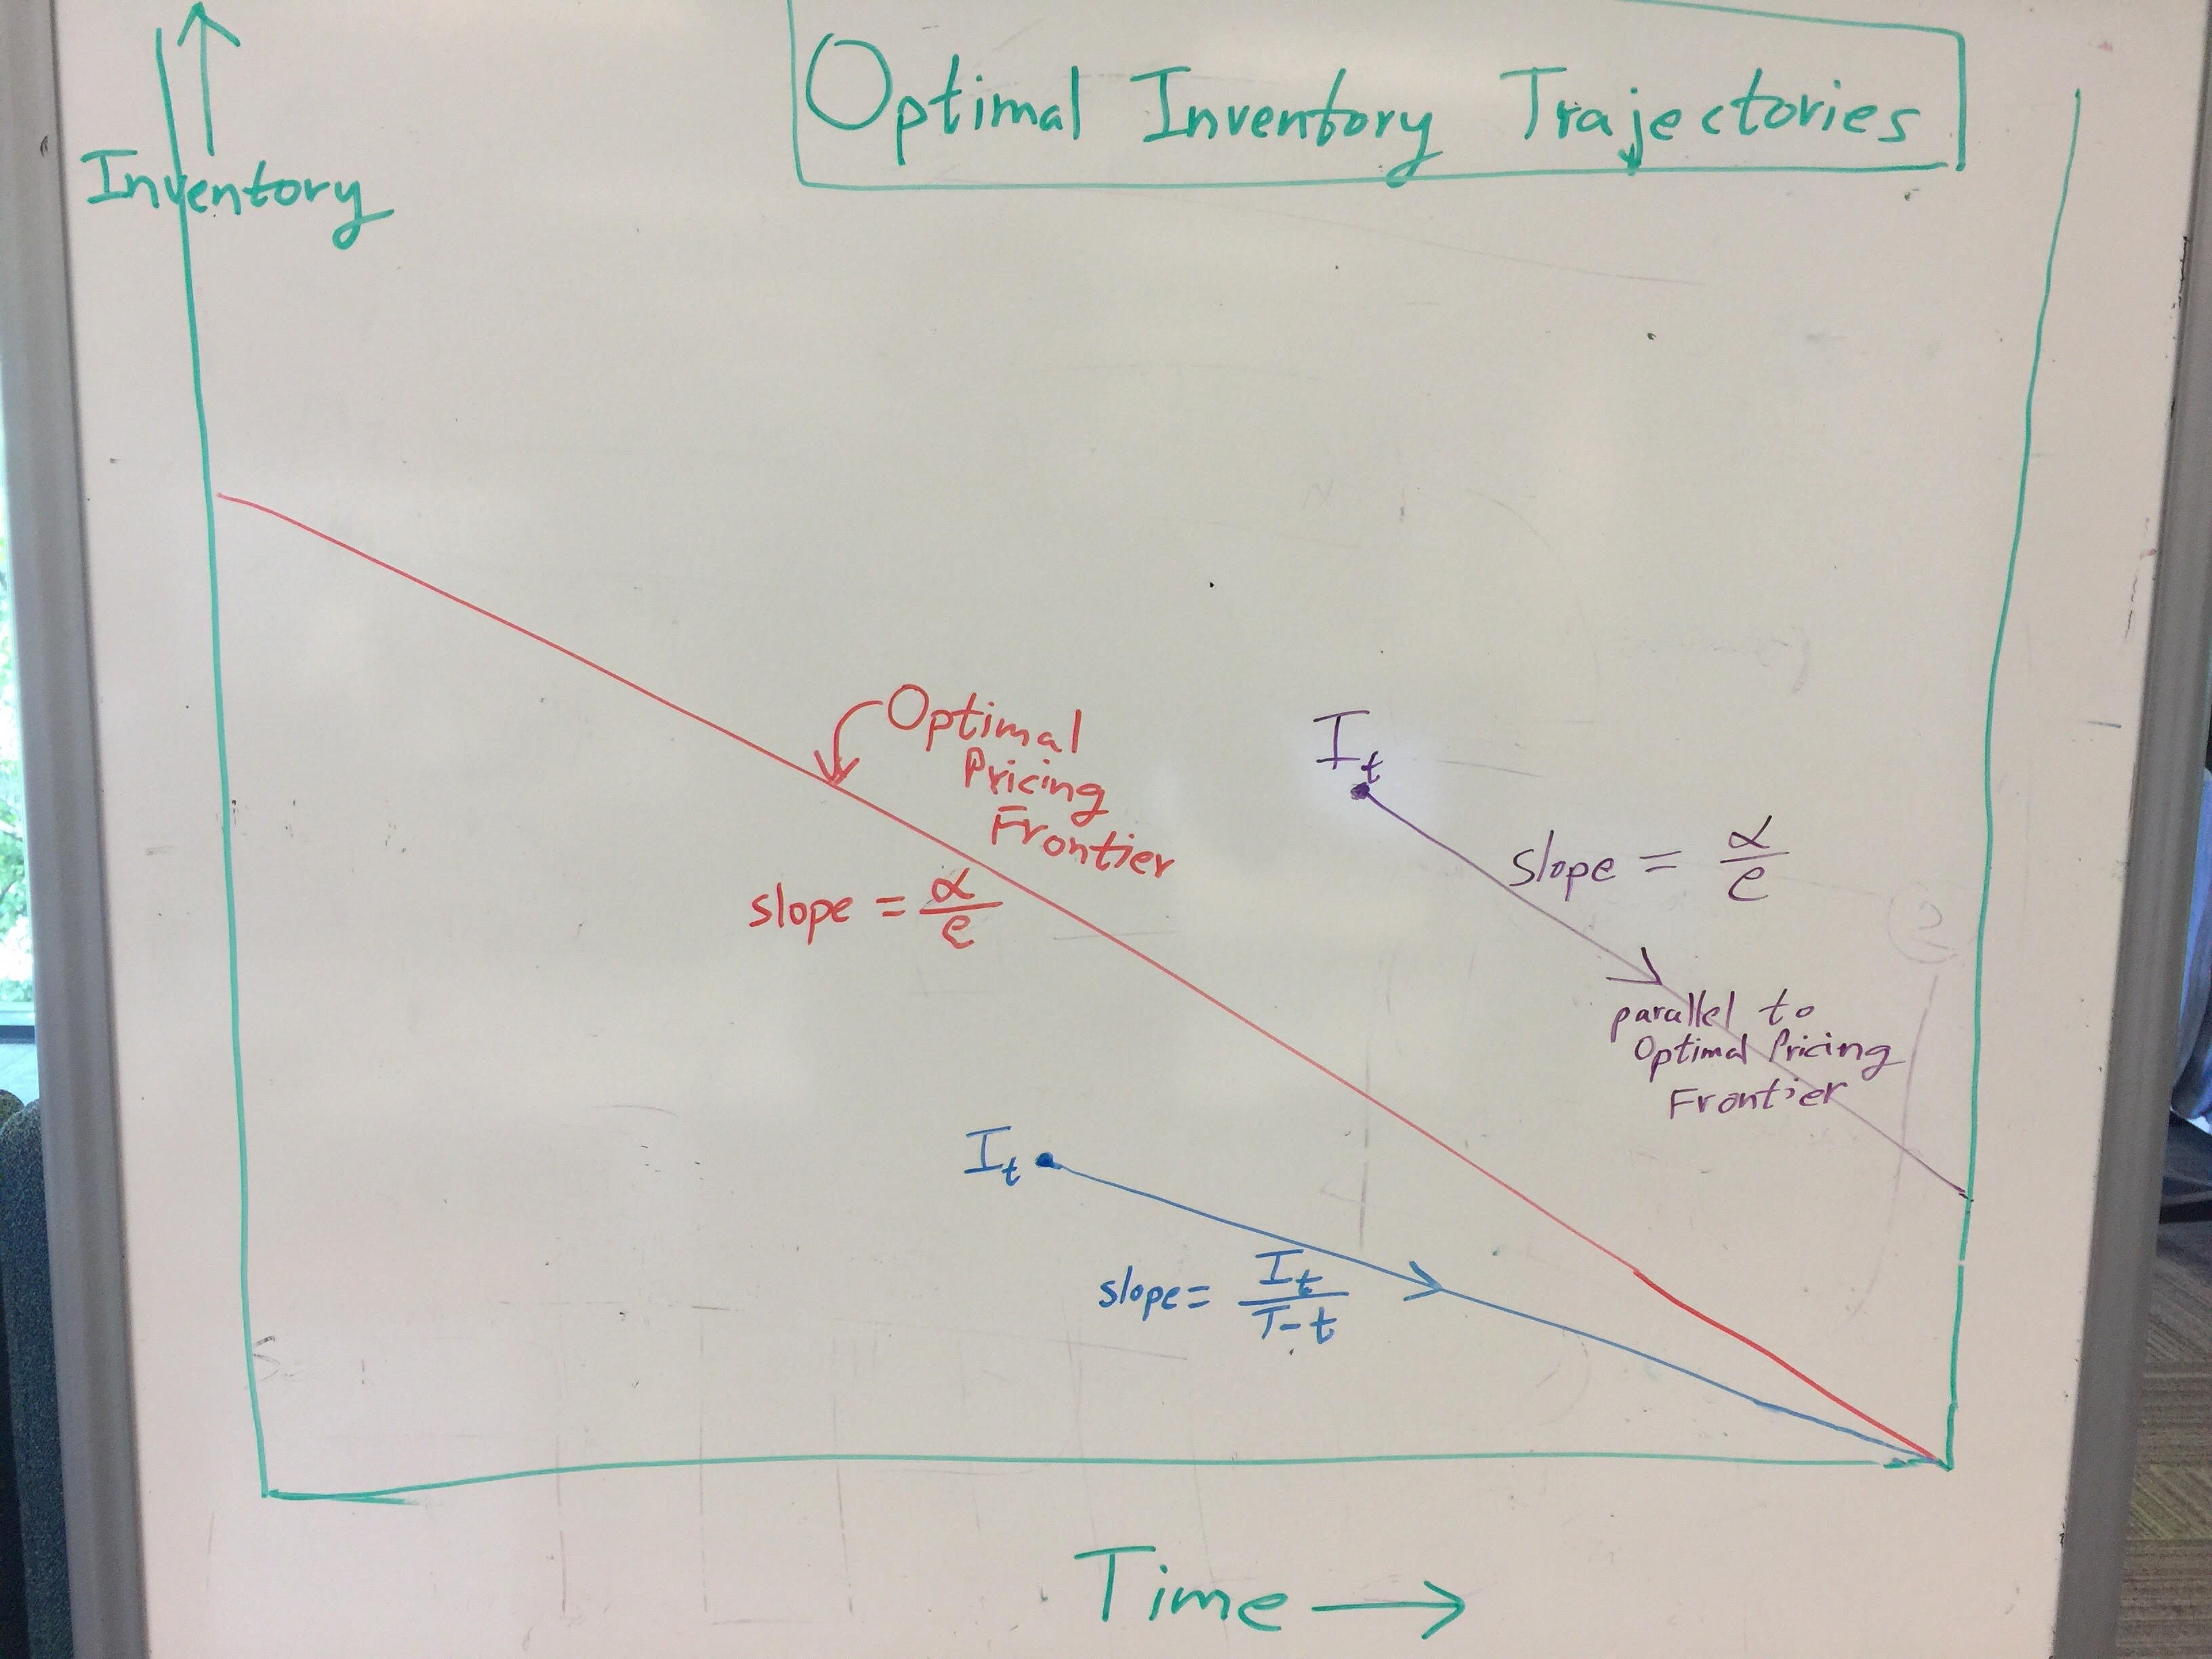
\includegraphics[width=0.82\textwidth]{frontier.jpg}
  \caption{Optimal Pricing Frontier}
\end{figure}

We note that:
\begin{itemize}
\item Above the ``Optimal Pricing Frontier'', Demand (under Optimal Pricing) occurs at the rate of $\frac \alpha e$ per time step (i.e., inventory trajectory is a straight line parallel to the ``Optimal Pricing Frontier''). We will refer to this Demand rate as the {\em Above Demand Rate}. Note that each unit of inventory above the ``Optimal Pricing Frontier'' is a unit that will remain unsold at the end of the clearance program.
\item Below the ``Optimal Pricing Frontier'', Demand (under Optimal Pricing) occurs at the rate of $\frac {I_t} {T-t}$ per time step (i.e., inventory trajectory is a straight line taking the inventory to exactly 0 at $t=T$). We will refer to this Demand rate as the {\em Below Demand Rate}.
\end{itemize}

Hence, the demand rate (under Optimal Pricing) is higher above the ``Optimal Pricing Frontier'', and correspondingly Optimal Price is lower above the ``Optimal Pricing Frontier'' (as expected). 
   
 \section{Calibration to ``Demand Lift'' (for Deterministic case)}
   
Let us assume that the ``base price'' is 1, for which the demand is $D_0$ (we will refer to $D_0$ as the {\em Base Demand}). Let us assume that the demand for ``half price off'' (i.e., for price of 0.5) is $D_{0.5} = (1+L)\cdot D_0$ (we will refer to $L$ as the {\em Demand Lift}). Let us calibrate the function $f(p) = \alpha \cdot e^{-\beta \cdot p}$ to these values:
   
$$D_0 = \alpha \cdot e^{-\beta}, D_{0.5} = \alpha \cdot e^{-\frac {\beta} 2}$$
Solving for $\alpha$ and $\beta$:
$$\alpha = \frac {D_{0.5}^2} {D_0} = D_0 \cdot (1+L)^2$$
$$\beta = 2 \log{(\frac {D_{0.5}} {D_0})} = 2 \log{(1 + L)}$$
$$f(p) = D_{0.5}^{2(1-p)} \cdot D_0^{2p-1} = D_0 \cdot (1+L)^{2(1-p)}$$

So, the ``Optimal Price Frontier'' (for the case of Deterministic Demand) is given by the line:
$$I_t = \frac {(T-t) \cdot D_0 \cdot (1+L)^2} {e}$$
Above the ``Optimal Price Frontier'', we have:
$$p_t^*(I_t) = \frac 1 {2 \log{(1+L)}}$$
$$V_t^*(I_t) = \frac {(T-t) \cdot D_0 \cdot (1+L)^2} {2 \cdot e \cdot \log{(1+L)}} $$

Below the ``Optimal Price Frontier'', we have:
$$p_t^*(I_t) = 1 + \frac {\log \frac {(T-t)D_0} {I_t}} {2 \log (1+L)}$$
$$V_t^*(I_t) = I_t(1 + \frac {\log \frac {(T-t)D_0} {I_t}} {2 \log (1+L)}) $$

\section{Qualitative Insights (for Deterministic case)}

\begin{itemize}
\item The {\em Above Price} is independent of inventory, independent of the {\em Base Demand}, and independent of time. The {\em Above Price} only depends on the {\em Demand Lift}. The greater the {\em Demand Lift}, the deeper the clearance price cuts.
\item The {\em Below Price} depends on the ratio of {\em Base Demand} to inventory and on the {\em Demand Lift}. The greater the inventory, the deeper the clearance price cuts. The smaller the {\em Base Demand}, the deeper the clearance price cuts. The greater the {\em Demand Lift}, the deeper the clearance price cuts.
\item The {\em Above Demand Rate} is independent of inventory and independent of time. The {\em Above Demand Rate} is sly increasing in the {\em Base Demand} and quadratically increasing in the {\em Demand Lift}.
\item The {\em Below Demand Rate} is independent of the {\em Base Demand} and independent of the {\em Demand Lift}. The {\em Below Demand Rate} is simply the ratio of inventory to remaining time (since we sell down to 0 exactly at the end of the clearance program).
\item The Optimal Value Function (Optimal Revenue in clearance program) above the ``Optimal Pricing Frontier'' is independent of inventory, linearly increasing in {\em Base Demand for the course of the program} and is an increasing function of the {\em Demand Lift}. So for a 10\% increase in {\em Base Demand}, we will get a 10\% increase in Revenue. For a practical value of {\em Demand Lift} $L = 1$ (i.e., 100\% increase in demand for a 50\% price cut), a 10\% increase in {\em Demand Lift} will fetch us a 3\% increase in Revenue.
\item The Optimal Value Function (Optimal revenue in clearance program) below the ``Optimal Pricing Frontier'' is an increasing function of inventory, an increasing function of the {\em Base Demand for the course of the program} (more demand results in lesser price cuts without lowering sales), and a decreasing function of {\em Demand Lift} (more lift results in greater price cuts without raising sales).
\end{itemize}
   
     
   \end{document}